\section{Evaluations}
\label{evaluation}

In this section, we evaluate our proposed index structure for k-truss community queries on real-world networks.

%\subsection{Datasets}
\vskip 0.1in \noindent \textbf{Datasets} 

\begin{table}
		\caption{Datasets}
		\vspace{2 mm}
		\label{table:datasets}
		\begin{threeparttable}
			\centering
			\begin{tabular}{c|ccccc} \hline
				Dataset & Type & $|V_{wcc}|$ & $|E_{wcc}|$ & $|\triangle|$ & $k_{max}$ \\ \hline
				Wiki & Communication & 2.4M & 4.7M &  & \\ 
				Skitter & Internet & 1.7M & 11.1M & & \\ 
				Livejournal & Social & 4.8M & 43.4M & & \\ 
				%Hollywood & Collaboration & 1.1M & 56.3M & & \\ 
				Orkut & Social & 3M & 117M & & \\ 
				Sinaweibo & Social & 58.7M & 261.3M & & \\ \hline
				%Webuk & Web & 39.3M & 796.4M & & \\ 
				%Friendster & Social & 65M & 1.8B & & \\ \hline
			\end{tabular}
			\begin{tablenotes}
				\item Datasets with the number of vertices and edges in the largest weakly connected components, the number of triangles and the maximum trussness of the graph.
			\end{tablenotes}
		\end{threeparttable}
\end{table}

We evaluate our algorithm on 5 graphs from different disciplines as shown in table~\ref{table:datasets}. To simplify our experiments, we treat them as undirected, un-weighted graphs and only use the largest weakly connected component of each graph. All datasets are collected from Stanford Network Analysis Project~\cite{snapnets} and Network Repository~\cite{nr-aaai15}.

%\subsection{Experiment settings}
\vskip 0.1in \noindent \textbf{Experiment settings} 

We evaluate our algorithms, we use a Cloudlab~\cite{RicciEide:login14} c8220 server with two 10-core 2.2GHz E5-2660 processors and 256GB memory. All algorithms are implemented in C++. 

\subsection{Query time}
\label{eval_query_time}

We evaluate the query time of various types of k-truss community queries on our index structure. We first evaluate the single vertex k-truss community search and compare the query time with the TCP index proposed in~\cite{huang2014querying}. We also use index free scheme as a baseline. As the k-truss community search time heavily rely on the degree of the query vertex, so we follow the similar procedure used in~\cite{huang2014querying}. We partition the vertices in each graph according to their degree into 10 categories and at each category, we randomly select 100 vertices to perform 100 independent k-truss community search. For all the queries, we fix the k at 10, which results in communities sufficiently large when degree of the query vertex is high to show the performance difference of different algorithms. For each query vertex, we first perform k-truss community identity search to find identity and seed edge for each resulting community on top-level index, and then we perform the k-truss community search on bottom-level index with breath first search.

\begin{figure}[ht]
    \centering
    %\includegraphics[width=\linewidth]{./figures/single_v_query_degree.pdf}
		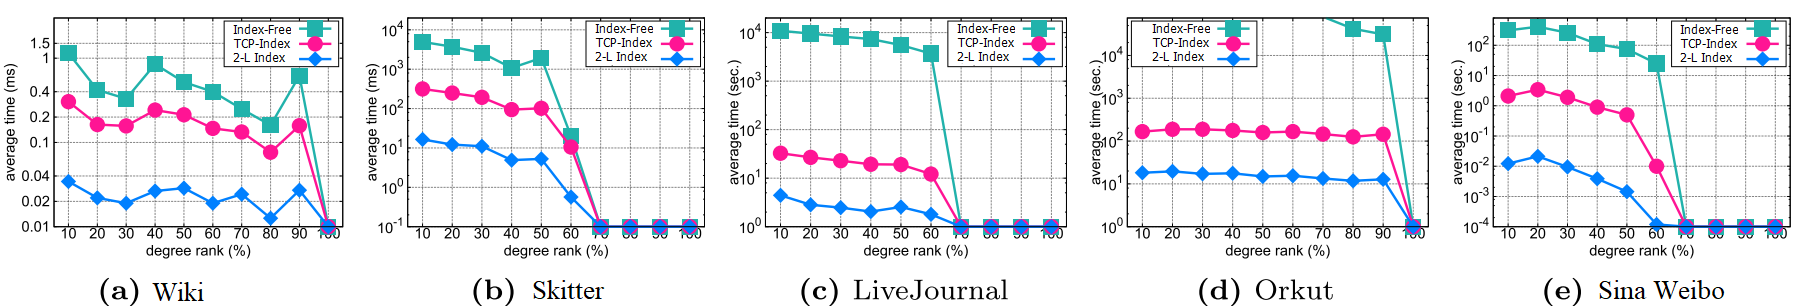
\includegraphics[width=\linewidth]{./figures/example1.png}
    \caption{Single vertex query for exact truss community search.}
    \label{fig:single_v_query_degree}
\end{figure}

We show the results for single vertex k-truss community search in figure \ref{fig:single_v_query_degree}. The results show that our index outperforms the TCP index proposed in~\cite{huang2014querying} by at least an order of magnitude. And both index scheme outperform the index-free method by sevearl orders of magnitude. Because the algorithm get rid of costly triangle connectivity discovery at query time and use straight forward edge connectivity by performing breath first search. 
 
\subsection{Index construction time and size}
\label{eval_const}

\begin{table}
		\caption{Comparison of Index Construction}
		\vspace{2 mm}
		\label{table:index_construction}
		\centering
		\begin{tabular}{|c|c|cc|cc|} \hline 
			 & Graph & \multicolumn{2}{|c|}{Index Size} & \multicolumn{2}{|c}{Index Time} \\
			\cline{3-6}
			Dataset & Size & TCP  & Our & TCP & Our \\ \hline
			Wiki & 57 & 296 & 187 & 138 & 117\\ 
			Skitter & 149 & 485 & 430 & 873 & 682\\ 
			Livejournal & 635 & 3174 & 2699 & 1686 & 1557\\ 
			%Hollywood & 791 & 4628 & 4012 & 4788 & 3966\\ 
			Orkut & 1769 & 8174 & 5742 & 3342 & 2884\\ 
			Sinaweibo & 4050 & 9322 & 7689 & 7730 & 6938 \\ \hline
			%Webuk & 13999 &   &  &  & \\ 
			%Friendster & 32364 &   &  &  & \\ \hline
		\end{tabular}
\end{table}

We show in this section the index size and index construction time of our scheme compared to TCP-index in 
table \ref{table:index_construction}. Both indices are generated in memory and we show the size of the data structures that hold the index. We exclude the truss decomposition time for both scheme so that the index construction time only shows how long it takes to generate a certain index with edge trussness provided.  We can see in table \ref{table:index_construction} that our scheme have smaller index size for most graphs and takes shorter time to generate the index compared to the TCP-index. Note that the index size contains both level of index structures. If only the k-truss community identity search is required, then the index size required for performing online queries is much smaller than the number provided here.

%\subsection{Index update time}
%\label{eval_update}
%
%The index update time upon graph changes, i.e. edge deletion, is shown in ... 


